\section{Gulp.js}
\label{gulpjs}

\textbf{Gulp.js} ist das GNU/Make für Node.js-Anwendungen. Als Task Runner führt Gulp repetitive Aufgaben im Web-Development, wie Linting, Unit-Testing, Code-Optimierung und -Kompilierung aus.

\subsection{gulpfile.js}

Das gulpfile ist eine Datei in einem Projekt, welches die einzelnen Aufgaben, deren Auslöser und Ausführung definiert. Aufgaben werden in Gulp mit \lstinline{gulp.task(name, runner)} definiert. So kann beispielsweise eine Build-Funktion für ein TypeScript-Projekt definiert werden:

\begin{code}[htp]
    \begin{center}
        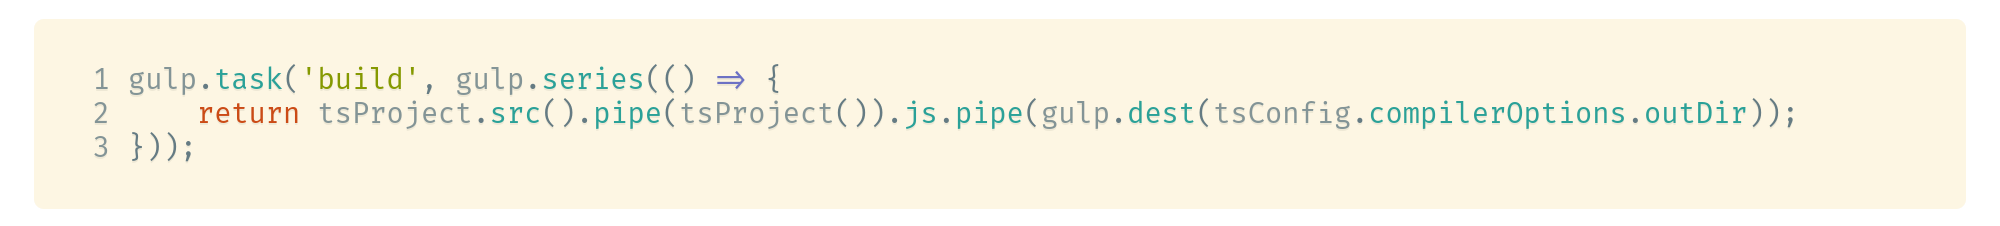
\includegraphics[width=1\textwidth]{images/Dependencies/gulpfile.png}
        \vspace{-25pt}
        \caption{Beispielhaftes \lstinline{gulpfile.js} zum Kompilieren von TypeScript}
    \end{center}
\end{code}

\subsection{Rolle von Gulp in Sokka}

Das \textit{Sokka-\nameref{backend}} nutzt Gulp.js für:

\begin{itemize}
    \item das \textbf{Kompilieren} von TypeScript-Code zu JavaScript-Code
    \item das \textbf{Überwachen} von Änderungen im TypeScript-Code (eine Änderung führt automatisch den \lstinline{build}-Task aus, via \lstinline{gulp-nodemon}-Plugin)
    \item das \textbf{Ausführen} bzw. \textbf{Debugging} vom Server
\end{itemize}